\section{Einleitung}

\subsection{Aufgabenstellung}

In folgenden wird die Implementierung einer abstrakten Datenstruktur für eine Client/Server Anwendung (siehe \ref{fig:nachrichtendienst}) behandelt. 

Die Aufgabe dieser Anwendung ist es Tagesnachrichten von verschiedenen Redakteuren zu verwalten und in korrekter Reihenfolge an den Kunden auszuliefern. Da die Reihenfolge der Nachrichten nicht von den Redakteuren abgestimmt wird, würde diese ohne einen Zwischenserver nicht korrekt sein. Die Nachrichten werden also von dem Redakteur-Client-Programm mit einer eindeutigen Nummerierung zuerst an einen Server gesendet. Dieser wird über das abstrakte Datenstruktur-Konzept einer Delivery und Holdback Queue verwaltet. Das heißt, dass zuerst alle Nachrichten in der Holdback Queue gehalten und nur bei korrekter Nummer an die Delivery Queue weitergegeben werden.\\ 
Von der Delivery Queue aus werden die Nachrichten auf Anfrage des Lesers dann in korrekter Reihenfolge an das entsprechende Client-Programm geschickt.\\
Da es auch hier wieder verschiedene Leser gibt hat der Server die Aufgabe sich für jeden Leser, insofern dieser sich nicht zu lange nicht mehr gemeldet hat, zu merken, welche Nachrichten er schon an diesen verschickt hat. 
Um den korrekten Ablauf der Anwendung kontrollieren zu können und um beim Implementieren Fehler möglichst einfach eliminieren zu können, werden alle Ausgaben in einer Datei HB-DLQ<Node>.log geschrieben.

Da die beiden Client Programme für die Redakteure und Leser zur Verfügung gestellt wurden, wird es im folgenden um die Implementierungen der Holdback und der Delivey Queue gehen.\\ 
Diese wird komplett in der funktionalen Programmiersprache Erlang umgesetzt und die beiden Dateien hbq.erl und dlq.erl enthalten den Code für die beiden Queues.  

\begin{figure}[htbp]
\begin{center}
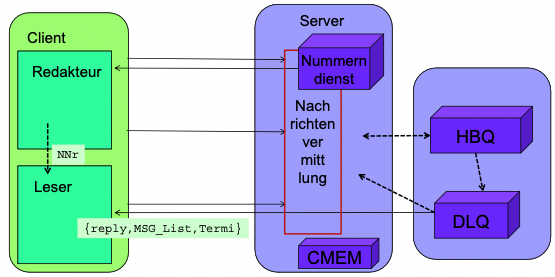
\includegraphics[scale=0.6]{Bilder/NachrichtendienstAbb.png}
\caption{\label{fig:nachrichtendienst} Nachrichtendienst \cite{Klauck2021}} 
\end{center}
\end{figure}

\subsubsection{Holdback Queue}

Die Holdback Queue enthält alle Nachrichten, die nicht ausgeliefert werden dürfen. Das heißt, dass die enthaltenen Nachrichten nicht die richtigen Nummern haben für die Delivery Queue haben. Durch regelmäßiges Prüfen wird entschieden, ob inzwischen eine geeignete Nachricht für die Delivery Queue von den Redakteuren empfangen wurde. 

Da die Nachrichten nach aufsteigender Nummerierung an die Delivery Queue weitergeleitet werden, bietet es sich an diese in der Holdback Queue bereits zu sortieren. 
Um diese Sortierung möglichst effizient zu gestalten werden verschiedene Algorithmen getestet (siehe Kapitel \ref{Problemstellungen}.).

\subsubsection{Nachrichten}

Nachrichten werden von den Redakteuren entwickelt und von den Lesern konsumiert. Bis sie beim Leser ankommen, können sie aber durch mögliche Software Fehler, wie z.B. asynchrone Nebenläufigkeiten oder ähnliches, verloren gehen. 
Die Nachrichten sind Tupel mit mindestens drei Elementen. Zum einen enthalten sie die Nachrichten-Nummer, nach welcher die Nachrichten sortiert werden. Dann enhalten sie eine Textzeile in welcher die eigentliche Nachricht geschrieben steht. Und abhängig davon, welche Queues sie schon durchlaufen haben, enthalten sie Zeitstempel mit den enstsprechenden Eintrittszeitstempeln. 

\subsection{Einfluss der Nebenläufigkeit}

Bedingt durch die Anzahl der Redakteure und Leser muss das Versenden und Empfangen der Nachrichten nebenläufig ausgeführt werden. In Erlang wird dies über Laufzeitsysteme mit verschiedenen Nodes umgesetzt. Die Holdback Queue wird somit ihrem eigenen Node zugewiesen und muss dadurch als entfernte abstrakte Datenstruktur implementiert werden. 

//TODO: Schnittstellen erklären

//TODO: auf Nebenläufigkeit eingehen

//TODO: Ablauf der Aufgabenerarbeitung (Entwurf, Impl, Tests, Messungen, Vergleiche, etc.)


